\begin{tcolorbox}[
        colbacktitle=colorrds!50!white,
        colback=colorrds!5!white,
        fonttitle=\bfseries,
        coltitle=black,
        colframe=colorrds!35!white,
        center title,
        adjusted title={Ángulos entre una secante y dos rectas paralelas}]
    \begin{tcbitemize}[raster columns=3, raster equal height=rows,
            size=small,coltitle=black,colback=white,
            colframe=colorrds!35!white,colbacktitle=gray!20,
            fonttitle=\centering\bfseries]
        \tcbitem[title=Ángulos Colaterales]
        \begin{figure}[H]
            \centering
            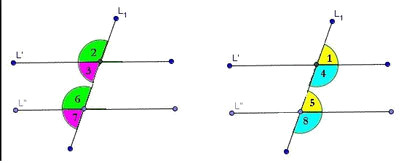
\includegraphics[width=\linewidth]{../images/angulos_colaterales.jpg}
            \caption{Son los ángulos que están ubicados al mismo lado de la secante.}
            \label{fig:angulos_colaterales}
        \end{figure}
        \tcbitem[title=Ángulos Internos]
        \begin{figure}[H]
            \centering
            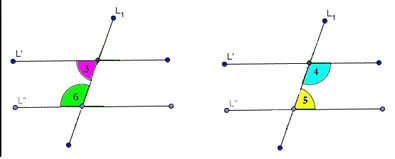
\includegraphics[width=\linewidth]{../images/angulos_internos.jpg}
            \caption{Son los ángulos que están ubicados entre las rectas paralelas.}
            \label{fig:angulos_internos}
        \end{figure}
        \tcbitem[title=Ángulos Externos]
        \begin{figure}[H]
            \centering
            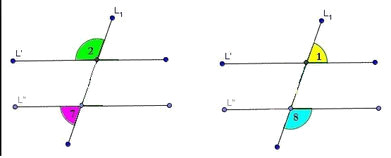
\includegraphics[width=\linewidth]{../images/angulos_externos.jpg}
            \caption{Son los ángulos que están ubicados por fuera de las rectas paralelas.}
            \label{fig:angulos_externos}
        \end{figure}
        \tcbitem[title=Ángulos Alternos Internos]
        \begin{figure}[H]
            \centering
            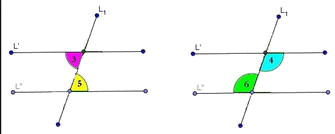
\includegraphics[width=\linewidth]{../images/angulos_alternos_internos.jpg}
            \caption{Son dos ángulos internos que no son colaterales ni adyacentes.}
            \label{fig:angulos_alternos_internos}
        \end{figure}
        \tcbitem[title=Ángulo Alternos Externos]
        \begin{figure}[H]
            \centering
            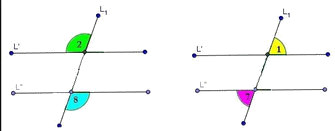
\includegraphics[width=\linewidth]{../images/angulos_alternos_externos.jpg}
            \caption{Son dos ángulos externos que no son colaterales ni adyacentes.}
            \label{fig:angulos_alternos_externos}
        \end{figure}
        \tcbitem[title=Ángulos Correspondientes]
        \begin{figure}[H]
            \centering
            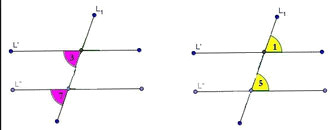
\includegraphics[width=\linewidth]{../images/angulos_correspondientes.jpg}
            \caption{Son dos ángulos uno interno y el otro externo que son colaterales pero no adyacentes.}
            \label{fig:angulos_correspondientes}
        \end{figure}
    \end{tcbitemize}
\end{tcolorbox}